\documentclass[11pt,a4paper]{article}

\usepackage[margin=25mm,headheight=14pt]{geometry}
\usepackage[T1]{fontenc}
\usepackage[utf8]{inputenc}
\usepackage{lmodern}
\usepackage{microtype}
\usepackage{amsmath,amssymb,mathtools}
\usepackage{booktabs,tabularx,longtable,array}
\usepackage{xcolor}
\usepackage{listings}
\usepackage{enumitem}
\usepackage{fancyhdr}
\usepackage{titlesec}
\usepackage{hyperref}
\usepackage{tikz}
\usetikzlibrary{arrows.meta,positioning}

\definecolor{navy}{HTML}{15324B}
\definecolor{blue}{HTML}{246A91}
\definecolor{pale}{HTML}{EEF4F8}
\definecolor{ink}{HTML}{202A33}
\definecolor{muted}{HTML}{52616B}
\definecolor{codebg}{HTML}{F4F6F8}
\definecolor{codegreen}{HTML}{287A55}
\definecolor{codepurple}{HTML}{7651A1}

\hypersetup{
  colorlinks=true,
  linkcolor=blue,
  urlcolor=blue,
  citecolor=blue,
  pdftitle={Argumentation Engine and Strategic Argumentation},
  pdfauthor={Sarah Fatima, Sahil Narkhede, Namya Dhingra, Anshit Agarwal},
  pdfsubject={Dung argumentation semantics and strategic argumentation}
}

\pagestyle{fancy}
\fancyhf{}
\fancyhead[L]{\small\color{muted}Argumentation Engine}
\fancyhead[R]{\small\color{muted}Autonomous Systems Assignment}
\fancyfoot[C]{\small\color{muted}\thepage}
\renewcommand{\headrulewidth}{0.4pt}
\renewcommand{\headrule}{\hbox to\headwidth{\color{blue}\leaders\hrule height \headrulewidth\hfill}}

\titleformat{\section}{\Large\bfseries\color{navy}}{\thesection}{0.7em}{}
\titleformat{\subsection}{\large\bfseries\color{blue}}{\thesubsection}{0.7em}{}
\titleformat{\subsubsection}{\normalsize\bfseries\color{navy}}{\thesubsubsection}{0.7em}{}
\setlist[itemize]{leftmargin=1.5em,itemsep=3pt,topsep=4pt}
\setlist[enumerate]{leftmargin=1.8em,itemsep=3pt,topsep=4pt}
\setlength{\parskip}{5pt}
\setlength{\parindent}{0pt}
\renewcommand{\arraystretch}{1.15}

\lstdefinestyle{python}{
  language=Python,
  basicstyle=\ttfamily\small,
  keywordstyle=\color{blue}\bfseries,
  commentstyle=\color{codegreen}\itshape,
  stringstyle=\color{codepurple},
  backgroundcolor=\color{codebg},
  frame=single,
  rulecolor=\color{black!12},
  numbers=left,
  numberstyle=\tiny\color{muted},
  numbersep=8pt,
  showstringspaces=false,
  breaklines=true,
  columns=fullflexible,
  keepspaces=true,
  tabsize=4,
  xleftmargin=1.5em,
  framexleftmargin=1.2em,
  aboveskip=8pt,
  belowskip=8pt
}
\lstdefinestyle{shell}{
  basicstyle=\ttfamily\small,
  backgroundcolor=\color{codebg},
  frame=single,
  rulecolor=\color{black!12},
  numbers=none,
  showstringspaces=false,
  breaklines=true,
  columns=fullflexible,
  aboveskip=8pt,
  belowskip=8pt
}
\lstset{style=python}

\newcommand{\AF}{\mathit{AF}}
\newcommand{\Grounded}{E_{\mathrm{gr}}}
\newcommand{\Pref}{E_{\mathrm{pr}}}
\newcommand{\Stable}{E_{\mathrm{st}}}
\newcommand{\Range}{\operatorname{range}}
\newcommand{\Pow}{\mathcal{P}}
\newcommand{\code}[1]{\texttt{\small #1}}
\newcommand{\result}[1]{\textbf{\color{navy}#1}}

\begin{document}

\begin{titlepage}
\thispagestyle{empty}
\begin{tikzpicture}[remember picture,overlay]
  \fill[navy] (current page.north west) rectangle ([yshift=-8.2cm]current page.north east);
  \fill[blue] ([yshift=-8.2cm]current page.north west) rectangle ([yshift=-8.35cm]current page.north east);
\end{tikzpicture}
\vspace*{1.15cm}
{\color{white}\Large\bfseries AUTONOMOUS SYSTEMS\par}
\vspace{1.4cm}
{\color{white}\Huge\bfseries Argumentation Engine\par}
\vspace{0.25cm}
{\color{white}\LARGE and Strategic Argumentation\par}
\vspace{0.7cm}
{\color{white}\large Implementation, verification, and computational experiments\par}
\vspace{5.5cm}
\begin{minipage}{0.78\textwidth}
{\large\bfseries Submitted by}\par
\vspace{0.25cm}
Sarah Fatima \hfill B23EE1093\\
Sahil Narkhede \hfill B23CS1060\\
Namya Dhingra \hfill B23CS1040\\
Anshit Agarwal \hfill B23CS1087
\end{minipage}
\vfill
{\large\bfseries 12 November 2026\par}
\vspace{0.4cm}
{\color{muted}Pure Python implementation; reproducible with the standard library.\par}
\end{titlepage}

\pagenumbering{roman}
\begin{abstract}
This project implements a complete small-framework engine for Dung-style abstract argumentation and studies strategic reporting under the grounded direct argumentation mechanism. The framework engine computes admissible and complete sets, grounded, preferred, stable, and semi-stable extensions, legal in/out/undec labellings, and acceptance statuses. The strategic component evaluates reports, enumerates best responses, checks the truthfulness inequality of Theorem~5.3, and tests the odd-path condition of Theorem~5.4, including two explicit interpretations of paths in cyclic graphs.

The implementation is validated against the book's Examples~5.10 and~5.11, hand-constructed semantic cases, and randomized cross-checks. The experiments evaluate 1,000 random instances for each of three attack probabilities. For the main no-self-attack setting, the measured strategyproof fractions are 0.632, 0.317, and 0.126 for $p=0.15,0.25,0.35$, respectively. No sampled instance satisfied the Theorem~5.4 condition while failing strategyproofness. Conversely, many instances remained strategyproof even though the sufficient condition failed, illustrating that the condition is not necessary.
\end{abstract}

\tableofcontents
\clearpage
\pagenumbering{arabic}

\section{Overview and objectives}

An abstract argumentation framework represents arguments and directed attacks between them. The first objective is to provide a reusable implementation of the principal Dung semantics. The second objective is to implement the grounded direct argumentation mechanism and investigate whether an agent can improve its outcome by concealing arguments it owns.

\subsection{Assignment coverage}
\begin{table}[ht]
\centering
\small
\begin{tabularx}{\textwidth}{@{}p{0.28\textwidth}X@{}}
\toprule
\textbf{Requirement} & \textbf{Implementation} \\
\midrule
Framework and basic semantics & \code{af\_project/argumentation.py}: framework class, conflict-freeness, defence, characteristic function, admissibility, completeness, grounded and other extensions, labellings, acceptance. \\
Strategic mechanism and best responses & \code{af\_project/strategic.py}: induced revealed framework, grounded outcome, utility, and exhaustive best-response enumeration. \\
Theorems 5.3 and 5.4 & Two Theorem~5.3 checks, plus odd-path detection and witnesses for Theorem~5.4. \\
Book examples and errata & \code{af\_project/book\_examples.py} and the tests/demo cover Examples~5.10 and~5.11 and both assignment-noted misprints. \\
Experiments and explanation & \code{af\_project/experiments.py}, \code{run\_experiments.py}, \code{analyse.py}, and saved results in \code{af\_project/results/}. \\
Submission demonstration & \code{af\_project/demo.py}, \code{demo\_output.txt}, and \code{DEMO.md}. \\
\bottomrule
\end{tabularx}
\caption{Where each requested component is implemented.}
\end{table}

\section{Argumentation framework and semantics}

\subsection{Definitions}
An argumentation framework is a pair
\[
\AF=(A,R),
\]
where $A$ is a finite set of arguments and $R\subseteq A\times A$ is the attack relation. We write $aRb$ when $a$ attacks $b$. For $S\subseteq A$, define the set attacked by $S$ as
\[
S^+=\{b\in A:\exists a\in S,\ (a,b)\in R\}.
\]
The set of attackers of an argument $a$ is $\operatorname{Att}(a)=\{b\in A:(b,a)\in R\}$.

\begin{description}[style=nextline,leftmargin=2.6cm,labelwidth=2.4cm]
\item[Conflict-free] $S$ is conflict-free iff no attack has both endpoints in $S$; self-attacks therefore make a set containing that argument non-conflict-free.
\item[Defence] $S$ defends $a$ iff each attacker of $a$ is attacked by at least one member of $S$. An unattacked argument is defended by every set, including the empty set.
\item[Characteristic function] $F(S)=\{a\in A:S\text{ defends }a\}$.
\item[Admissible] $S$ is conflict-free and $S\subseteq F(S)$.
\item[Complete] $S$ is conflict-free and $S=F(S)$.
\item[Grounded] The grounded extension is the least fixed point of $F$, computed by iterating from the empty set.
\item[Preferred] An inclusion-maximal admissible set.
\item[Stable] A conflict-free set $S$ with $S\cup S^+=A$.
\item[Semi-stable] An admissible set whose range $S\cup S^+$ is inclusion-maximal among admissible sets.
\end{description}

The characteristic function is monotone. Starting from $\varnothing$, iteration reaches its least fixed point on a finite framework. The grounded extension is unique and is contained in every complete extension.

\subsection{Labellings and acceptance}
A labelling assigns one of \emph{in}, \emph{out}, or \emph{undec} to each argument. It is legal if, for every argument $a$:
\[
\begin{aligned}
a\text{ is in} &\iff \text{every attacker of }a\text{ is out},\\
a\text{ is out} &\iff \text{at least one attacker of }a\text{ is in},\\
a\text{ is undec} &\iff \text{no attacker is in and not all attackers are out}.
\end{aligned}
\]
Legal labellings correspond one-to-one with complete extensions via their in-labelled arguments. Labellings without undecided arguments correspond to stable extensions.

For a selected semantics, an argument is \emph{skeptically accepted} if it belongs to every extension, \emph{credulously accepted} if it belongs to some but not all extensions, and \emph{rejected} if it belongs to none. If stable semantics has no extension, the implementation reports an explicit undefined/no-extensions status instead of assigning one of these labels.

\subsection{Implementation approach}
The \code{ArgumentationFramework} object stores the argument set, attack relation, and precomputed attacker/target maps. Its constructor rejects attacks mentioning unknown arguments. Semantic computations use exhaustive subset enumeration, which is transparent and appropriate for the small frameworks in this assignment:
\begin{itemize}
\item up to $2^{|A|}$ candidate sets for extension semantics;
\item up to $3^{|A|}$ candidate labellings;
\item iteration of $F$ for the grounded extension.
\end{itemize}
The implementation also provides function-style wrappers around the class methods, so both object-oriented and function-oriented use are available.

\section{Strategic argumentation}

\subsection{Model and utility}
There are agents $i\in N$ with pairwise disjoint true argument sets $A_i$. A report is any subset $R_i\subseteq A_i$. Given public attack relation $R$, the mechanism forms the framework induced by the union of reports:
\[
M(R_1,\ldots,R_n)=
\Grounded\left(
\left(\bigcup_i R_i,\ R\cap\left(\bigcup_iR_i\right)^2\right)
\right).
\]
The utility of agent $i$ is the number of its true arguments accepted:
\[
u_i(R_1,\ldots,R_n)=|A_i\cap M(R_1,\ldots,R_n)|.
\]
Thus an agent cannot invent an argument, and arguments it owns but hides remain part of its utility type, but not of the reported graph. Truthful reporting is weakly optimal when no alternative report gives strictly greater utility; it need not be the unique best response.

\subsection{Mechanism and best response}
\code{mechanism(attacks, reports)} returns the grounded extension of the induced revealed framework. \code{best\_responses(agent, agents, attacks, others\_reports)} checks every subset of that agent's true arguments, evaluates the resulting grounded extension, and returns both the maximum utility and all reports attaining it. This exhaustive method gives a direct, auditable best-response calculation for small types.

\subsection{Theorem 5.3: truthfulness criterion}
For every agent $i$, every subset $S\subseteq A_i$ to hide, and every possible union $A_{-i}$ of other agents' reports, Theorem~5.3 requires
\[
\left|A_i\cap\Grounded\bigl(A_i\cup A_{-i},R\bigr)\right|
\ \geq\
\left|A_i\cap\Grounded\bigl((A_i\setminus S)\cup A_{-i},R\bigr)\right|.
\tag{1}\label{eq:theorem53}
\]
The code checks the equivalent best-response statement with a bitmask implementation and also provides a second, literal inequality implementation using the framework class. The tests compare the two approaches on randomized instances. Inputs to the exhaustive checks are validated: ownership sets must be disjoint, and every attack must mention arguments owned by an agent.

\subsection{Theorem 5.4: odd paths}
An odd-length directed path from $\alpha$ to $\beta$ is denoted $\alpha\rightsquigarrow\beta$. The sufficient condition checked here is that no agent owns two distinct arguments $\alpha,\beta$ with $\alpha\rightsquigarrow\beta$ in the full attack graph. The implementation returns both the violations and witness paths.

In cyclic graphs, the word path can be interpreted in two ways. The default \emph{walk} interpretation permits repeated vertices; the search is breadth-first over states $(v,\ell\bmod 2)$ and terminates because there are only $2|A|$ such states. The \emph{simple path} interpretation disallows repeated vertices and is checked separately. Reporting both makes the ambiguity visible rather than silently choosing one interpretation. The experimental headline uses the walk interpretation.

\section{Worked examples from the book}

\subsection{Example 5.10: hiding can increase utility}
The arguments are partitioned as
\[
A_x=\{a_1,a_4,a_5\},\qquad A_y=\{a_2\},\qquad A_z=\{a_3\},
\]
with attacks $a_1\to a_2$, $a_2\to a_3$, $a_3\to a_4$, and $a_3\to a_5$.

\begin{figure}[ht]
\centering
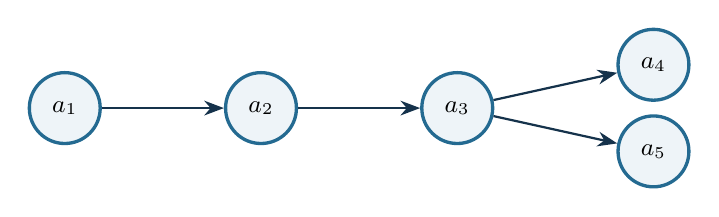
\begin{tikzpicture}[
  node distance=1.15cm and 1.55cm,
  arg/.style={circle,draw=blue,very thick,fill=pale,minimum size=9mm,font=\small\bfseries},
  attack/.style={-{Stealth[length=2.5mm]},thick,draw=navy}
]
\node[arg] (a1) {$a_1$};
\node[arg,right=of a1] (a2) {$a_2$};
\node[arg,right=of a2] (a3) {$a_3$};
\node[arg,right=of a3,yshift=0.55cm] (a4) {$a_4$};
\node[arg,right=of a3,yshift=-0.55cm] (a5) {$a_5$};
\draw[attack] (a1)--(a2);
\draw[attack] (a2)--(a3);
\draw[attack] (a3)--(a4);
\draw[attack] (a3)--(a5);
\end{tikzpicture}
\caption{Attack graph for Example 5.10.}
\label{fig:example510}
\end{figure}

When all agents report truthfully, the grounded extension is $\{a_1,a_3\}$. Utilities are $(u_x,u_y,u_z)=(1,0,1)$. If $x$ hides $a_1$, the revealed graph has grounded extension $\{a_2,a_4,a_5\}$, giving $x$ utility $2$. Truthful reporting is therefore not a best response against truthful reports by $y$ and $z$, and the mechanism is not strategyproof. The odd paths $a_1\to a_2\to a_3\to a_4$ and $a_1\to a_2\to a_3\to a_5$ also witness failure of the Theorem~5.4 condition.

\textbf{Correction of the stated misprint.} Example~5.10's utility discussion swaps $y$'s and $z$'s argument sets. Using each agent's actual set gives $u_y=0$ and $u_z=1$.

\subsection{Example 5.11: sufficient is not necessary}
Example~5.11 adds argument $a_6$ to $A_x$ and adds the attack $a_6\to a_3$. The truthful grounded extension is $\{a_1,a_4,a_5,a_6\}$ and all four of $x$'s arguments are accepted. The instance is strategyproof, although the odd paths from $a_1$ to $a_4$ and $a_5$ remain. This demonstrates that Theorem~5.4's condition is sufficient but not necessary.

\textbf{Correction of the stated misprint.} The argument that cancels the indirect self-defeat is $a_6$, not $a_5$. Revealing $a_6$ makes it accepted and attacks $a_3$, preventing the chain from using $a_3$ to defeat $a_4$ and $a_5$.

\section{Experiments}

\subsection{Protocol}
We generated instances with three agents and $n$ uniformly selected from $\{6,7,8\}$. For each ordered pair of distinct arguments, an attack is independently included with probability $p$. Each argument is independently assigned uniformly to one of the three agents; an agent may own no arguments. We used $p\in\{0.15,0.25,0.35\}$ and generated 1,000 instances for each $p$ (3,000 total), using seed 2024. Strategyproofness is tested exhaustively, not estimated by sampling deviations. A separate variant permits self-attacks.

The main experiment excludes self-attacks, matching the explicit restriction $a\ne b$ in the assignment's random attack model. The extra variant provides a sensitivity check for the ambiguous phrase ``each possible attack.''

\subsection{Strategyproofness rates}
\begin{table}[ht]
\centering
\begin{tabular}{@{}crr@{}}
\toprule
$p$ & No self-attacks & Self-attacks allowed \\
\midrule
0.15 & 632/1000 = \result{0.632} & 535/1000 = 0.535 \\
0.25 & 317/1000 = \result{0.317} & 254/1000 = 0.254 \\
0.35 & 126/1000 = \result{0.126} & 101/1000 = 0.101 \\
\bottomrule
\end{tabular}
\caption{Fraction of strategyproof instances for each attack probability.}
\label{tab:sp}
\end{table}

\begin{figure}[ht]
\centering
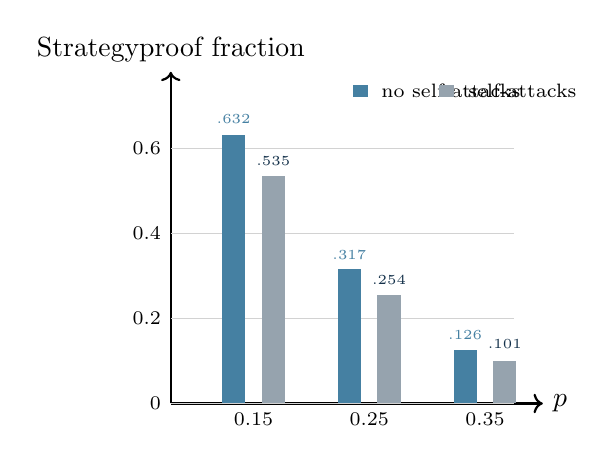
\begin{tikzpicture}[x=1.05cm,y=5.4cm]
\draw[->,thick] (0,0)--(4.5,0) node[right] {$p$};
\draw[->,thick] (0,0)--(0,0.78) node[above] {Strategyproof fraction};
\foreach \y/\lab in {0/0,0.2/0.2,0.4/0.4,0.6/0.6} {
  \draw[gray!35] (0,\y)--(4.15,\y);
  \node[left] at (0,\y) {\scriptsize \lab};
}
\foreach \x/\lab in {1/0.15,2.4/0.25,3.8/0.35} {
  \node[below] at (\x,0) {\scriptsize \lab};
}
\fill[blue!85] (0.62,0) rectangle (0.90,0.632);
\fill[blue!85] (2.02,0) rectangle (2.30,0.317);
\fill[blue!85] (3.42,0) rectangle (3.70,0.126);
\fill[navy!45] (1.10,0) rectangle (1.38,0.535);
\fill[navy!45] (2.50,0) rectangle (2.78,0.254);
\fill[navy!45] (3.90,0) rectangle (4.18,0.101);
\node[blue!85] at (0.76,0.67) {\tiny .632};
\node[navy] at (1.24,0.57) {\tiny .535};
\node[blue!85] at (2.16,0.35) {\tiny .317};
\node[navy] at (2.64,0.29) {\tiny .254};
\node[blue!85] at (3.56,0.16) {\tiny .126};
\node[navy] at (4.04,0.14) {\tiny .101};
\fill[blue!85] (2.2,0.72) rectangle (2.38,0.75);
\node[right] at (2.43,0.735) {\scriptsize no self-attacks};
\fill[navy!45] (3.25,0.72) rectangle (3.43,0.75);
\node[right] at (3.48,0.735) {\scriptsize self-attacks};
\end{tikzpicture}
\caption{Measured strategyproof rates. Rates decrease as attack density increases.}
\label{fig:rates}
\end{figure}

The measured fraction declines as the attack graph becomes denser. In these small random instances, denser attack relations create more opportunities for interactions between an agent's own arguments. However, the rates depend on the assignment and sampling model; they are not universal probabilities about argumentation frameworks.

\subsection{Theorem 5.4 condition versus strategyproofness}
\begin{table}[ht]
\centering
\small
\begin{tabular}{@{}crrrr@{}}
\toprule
$p$ & Condition holds (walk) & Holds but not SP & SP, condition fails (walk) & SP, condition fails (simple)\\
\midrule
0.15 & 118 & 0 & 514 & 512 \\
0.25 & 31 & 0 & 286 & 284 \\
0.35 & 4 & 0 & 122 & 121 \\
\bottomrule
\end{tabular}
\caption{Cross-tabulation for the main, no-self-attack experiment.}
\label{tab:thm54}
\end{table}

No sampled instance satisfied the condition yet failed strategyproofness, consistent with Theorem~5.4's sufficient-condition claim. This finite experiment is an empirical verification, not a proof. The number of condition-satisfying instances is small at high density, so the zero count at $p=0.35$ should be interpreted with that limitation in mind.

The condition is not necessary: 514, 286, and 122 instances at the three probabilities were strategyproof even under the default walk interpretation while violating the condition. This count includes cases where truthful reporting ties a deviation; such ties do not violate weak strategyproofness.

\subsection{Why can the condition fail while truth remains optimal?}
For every strategyproof instance that failed the walk condition, we compared the agent's accepted true arguments under truth and every strictly smaller report. We classify each instance by its most informative deviation:
\begin{itemize}
\item \textbf{Swap:} the accepted set changes but its size stays the same; the agent exchanges one accepted argument for another.
\item \textbf{Loss-only:} at least one deviation reduces utility, and no equal-utility swap occurs.
\item \textbf{Inert:} every deviation leaves the accepted set unchanged.
\end{itemize}
\begin{table}[ht]
\centering
\begin{tabular}{@{}crrrr@{}}
\toprule
$p$ & Strategyproof, condition fails & Swap & Loss-only & Inert\\
\midrule
0.15 & 514 & 445 & 69 & 0\\
0.25 & 286 & 243 & 43 & 0\\
0.35 & 122 & 103 & 19 & 0\\
\bottomrule
\end{tabular}
\caption{Classification of strategyproof instances that violate the walk condition.}
\label{tab:classification}
\end{table}

Most such instances contain a zero-sum swap. A short odd path can make it possible to release a same-agent argument by hiding another, but hiding also removes an argument from the reported framework. For example, with a single attack $\alpha\to\beta$ and both arguments owned by one agent, truth accepts $\alpha$ and rejects $\beta$. Hiding $\alpha$ can accept $\beta$ instead, leaving the utility unchanged. This violates the sufficient condition but does not make hiding profitable.

In a loss-only example, redundant blockers can prevent the hidden argument's removal from releasing a target. If two accepted attackers block an argument owned by the agent, hiding just one still leaves the other attack in place; hiding both can cost more utility than it gains. The condition tracks odd-path structure, not the net utility of every possible report, which explains why it can fail without a profitable deviation.

\subsection{A profitable deviation}
The smallest illustrative mechanism in the demonstration has agent 1 owning $\{\alpha,\beta\}$ and agent 2 owning $\{d,e\}$. The attacks are $\alpha\to\beta$, $\alpha\to d$, $d\to e$, and $e\to\alpha$. The truthful grounded outcome leaves agent 1 with utility 0; hiding $\alpha$ breaks the odd cycle and allows $\beta$ to be accepted, giving utility 1. This is a concrete case where the condition fails and the mechanism is not strategyproof.

\section{Verification and demonstration}

\subsection{Automated tests}
The standard-library test suite is \code{af\_project/tests.py}. It checks:
\begin{itemize}
\item hand-constructed chains, even and odd cycles, self-attacks, and examples distinguishing semantics;
\item the book's Examples~5.10 and~5.11, including the assignment's corrections;
\item 300 random frameworks for structural cross-checks, including grounded-as-least-complete and the correspondence between complete extensions and legal labellings;
\item the bitmask and class-based grounded mechanism implementations on random instances;
\item consistency between best-response enumeration and the truthfulness checker;
\item agreement between the two independent Theorem~5.3 implementations on 150 randomized instances;
\item odd-walk search against bounded brute-force enumeration on 100 random graphs, plus witness validity;
\item the Theorem~5.4 sufficient-condition implication on randomized checks.
\end{itemize}
The test command completed successfully with the final output \result{\code{ALL TESTS PASSED}}.

\subsection{Demonstration plan}
The live demonstration script \code{af\_project/demo.py} and guide \code{af\_project/DEMO.md} provide a concise walkthrough:
\begin{enumerate}
\item classic frameworks and their extensions and labellings;
\item Example~5.10, the profitable concealment, and the Theorem~5.3/5.4 checks;
\item Example~5.11, demonstrating that the Theorem~5.4 condition is not necessary;
\item examples where the condition holds and fails, and walk-versus-simple-path behavior on cycles.
\end{enumerate}

\section{Limitations and interpretation}
\begin{itemize}
\item The semantics and strategic checks are exhaustive and exponential. They are intended for the small frameworks in this assignment, not large-scale deployment.
\item The random experiment uses a specific model: uniformly chosen size from 6--8, independent assignment of each argument to one of three agents, and independent attacks. Agents may receive zero arguments.
\item The path definition on cyclic graphs has two plausible interpretations. Both are implemented and reported; the main condition uses walks, which allow repeated vertices.
\item Randomized experiments support reproducibility and reveal patterns, but cannot establish a theorem. Theorem~5.4's sufficiency is supported by its statement and checked exhaustively per sampled instance; this is not a formal proof.
\item Strategyproofness is weak: truth must be among the best reports, not the unique best report.
\end{itemize}

\section{Reproduction and project layout}
The project uses Python 3 and the standard library only. From the repository root:
\begin{lstlisting}[style=shell]
cd af_project
python tests.py
python demo.py
python run_experiments.py
\end{lstlisting}
The experiment runner accepts an optional instance count per probability. For example, \code{python run\_experiments.py 1000} runs 1,000 instances per $p$ and writes result tables and JSON data under \code{af\_project/results/}. Results use a fixed seed of 2024.

\begin{table}[ht]
\centering
\small
\begin{tabularx}{\textwidth}{@{}lX@{}}
\toprule
\textbf{Path} & \textbf{Purpose}\\
\midrule
\code{af\_project/argumentation.py} & Argumentation framework and semantics.\\
\code{af\_project/strategic.py} & Strategic mechanism, best responses, theorem checks.\\
\code{af\_project/book\_examples.py} & Encoded book examples and corrected notes.\\
\code{af\_project/tests.py} & Automated assertions and randomized cross-checks.\\
\code{af\_project/demo.py} & Runnable demonstration.\\
\code{af\_project/experiments.py} & Random instance generation and summaries.\\
\code{af\_project/results/} & Reproducible experiment summaries and instance records.\\
\code{README.md} & Project overview and usage instructions.\\
\end{tabularx}
\caption{Files included with the submission.}
\end{table}

\section{Conclusion}
The project delivers both requested parts: a working implementation of standard argumentation semantics and an exhaustive small-instance study of strategic reporting under the grounded mechanism. The implementation passes its tests and reproduces the book examples, including the specified corrections. In the experiments, strategyproofness becomes less common as attack density increases, while the Theorem~5.4 condition remains sufficient but is far from necessary. In most sampled strategyproof instances that violate the condition, concealment merely trades one accepted argument for another rather than increasing utility.

\end{document}
